\subsection{UC8 - Caricamento file JSON contenente i predittori}
\begin{figure}[H]
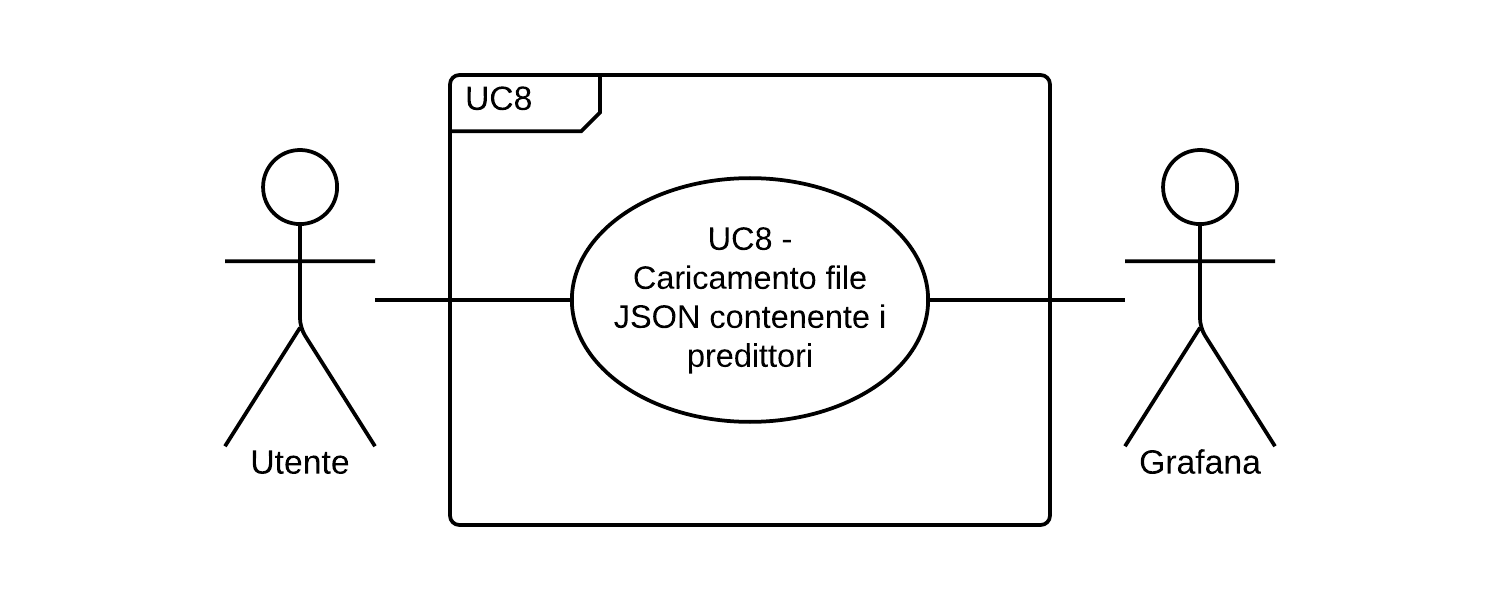
\includegraphics{img/UC8_-_Caricamento_file_JSON_contenente_i_predittori.png}
\caption{Diagramma degli use case di UC8}
\end{figure}
\begin{itemize}
	\item \textbf{Codice identificativo}: UC8;
	\item \textbf{Titolo}: caricamento file JSON contenente i predittori;
	\item \textbf{Attori primari}: utente;
	\item \textbf{Attori secondari}: Grafana\glo;
	\item \textbf{Descrizione}: l'utente esegue l'attività di caricamento del file JSON contenente i dati risultati dall'addestramento da utilizzare durante la previsione;
	\item \textbf{Precondizioni}: l'utente è autenticato nel sistema software Grafana\glosp, ha configurato una dashboard\glosp per la visualizzazione del risultato e ha avviato il plug-in;
	\item \textbf{Postcondizioni}: il file JSON contenente i dati risultati dall'addestramento è stato caricato correttamente;
	\item \textbf{Scenario principale}: l'utente carica il file JSON contente i dati risultati dall'addestramento.
\end{itemize}